%!TeX root=../tese.tex
%("dica" para o editor de texto: este arquivo é parte de um documento maior)
% para saber mais: https://tex.stackexchange.com/q/78101

%% ------------------------------------------------------------------------- %%

% "\chapter" cria um capítulo com número e o coloca no sumário; "\chapter*"
% cria um capítulo sem número e não o coloca no sumário. A introdução não
% deve ser numerada, mas deve aparecer no sumário. Por conta disso, este
% modelo define o comando "\unnumberedchapter".
\unnumberedchapter{Introduction}
\label{cap:introduction}

\enlargethispage{.5\baselineskip}

Weather and climate predictions are recognized as a good for mankind,
due to the information they yield for diverse activities. 
For instance, short-range forecasts are useful for public use, while
medium-range forecasts are helpful for industrial activities and agriculture. 
Seasonal forecasts (one up to three months) are important to energy planning and agriculture.
At last, longer-range forecasts (one century, for instance) are useful for climate change 
studies that are important for government planning.

Lat-lon models \citep{will:2007}...

The emergence of the Fast Fourier transform (FFT) in the 1960s with the work from 
\citet{cooley:1965} allowed the computation of discrete Fourier transforms with
$N\log(N)$ complexity. 
The viability of the usage of FFTs for solving atmospheric flows was shown by \citet{orszag:1970},
using the barotropic vorticity equation on the sphere, and by \citet{eliasen:1970}, using
the primitive equations.
The spectral method expresses latitude-longitude grid values, that represent some scalar field,
using truncated spherical harmonics expansions, which consists of Fourier expansions 
in latitude circles and Legendre functions expansions in longitude circles. 
The coefficients in the spectral expansions are known
as spectral coefficients and are usually thought to live in the so-called spectral space.
Given the grid values, the spectral coefficients are obtained by performing a FFT followed by a 
Legendre Transform (LT). 
Conversely, given the spectral coefficients,
the grid values are obtained by performing an inverse LT followed by an inverse FFT.
The main idea of the spectral method is to apply the spectral transform, in order to 
go the spectral space, and evaluate spatial derivatives in the spectral space, which
consists of multiplying the spectral coefficients by constants. 
Then, the method performs the inverse spectral transform
in order to get back to grid space, and the nonlinear terms are treated on the grid space
\citep{krishnamurti:2006}.

The dominance of spectral transform \citep{will:2007}.
Indeed, the spectral method is still used in many current operational Weather Forecasting models such as
the Integrated Forecast System (IFS) from  European Centre for Medium-Range Weather Forecasts (ECMWF),
Global Forecast System (GFS) from National Centers for Environmental Prediction (NCEP) and the
Brazilian Global Atmospheric Model (BAM) \citep{figueroa:16} from  Center for Weather Forecasting 
and Climate Research [Centro de Previsão de Tempo e Estudos Climáticos (CPTEC)]. 

With the beginning of the multicore era in the 1990's. 
The parallelization of the spectral method requires
data transposition, FFT and LT in parallel \citep{barros:1995}.
Requires a lot of communication using Message passing interface (MPI) \citep{mueller:2019} \citep{zheng:2018}

\newpage
\begin{figure}
  \centering
  \begin{subfigure}{.3\linewidth}
    \centering
    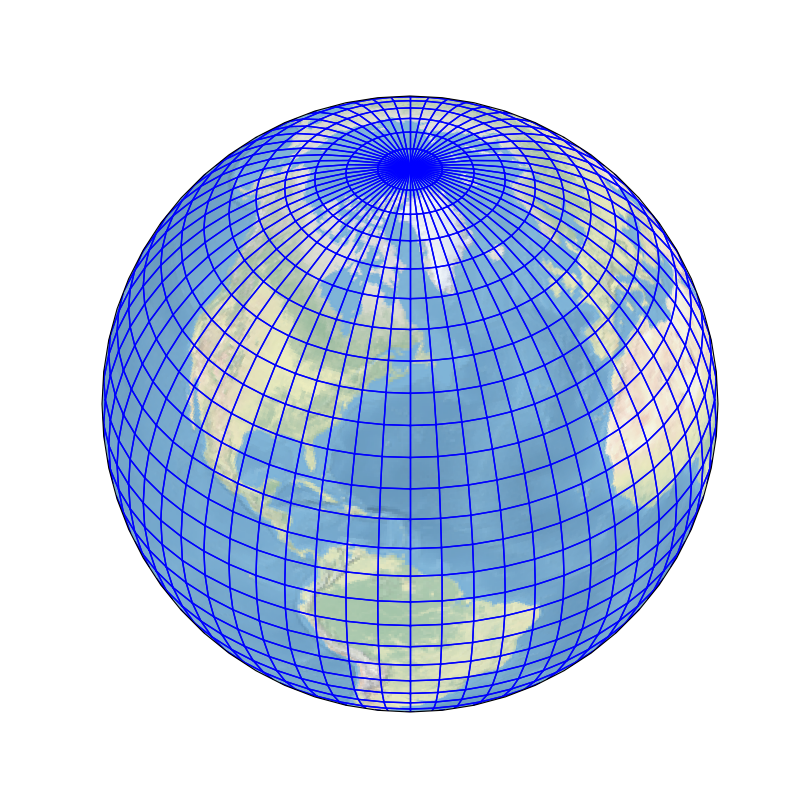
\includegraphics[width = \linewidth]{latlon_sphere}
      \caption{Latitude-longitude grid}\label{latlon-grid}
  \end{subfigure}%
  \hspace{1em}% Space between image A and B
  \begin{subfigure}{.3\linewidth}
    \centering
    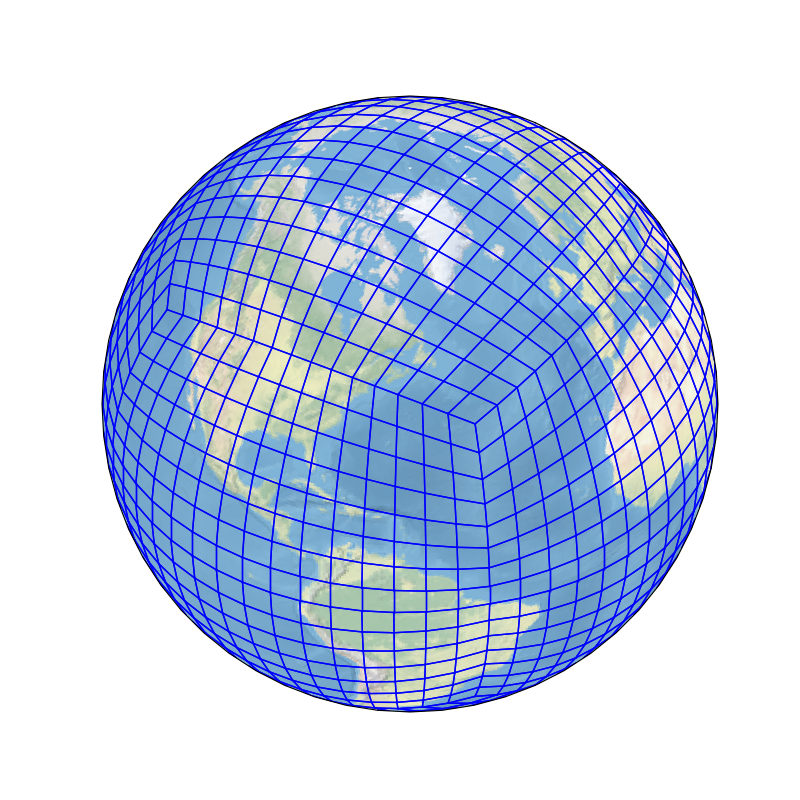
\includegraphics[width = \linewidth]{gnomonic_equiangular_15_sphere}
      \caption{Cubed-sphere}\label{cs-grid}
  \end{subfigure}%
  \hspace{2em}% Space between image B and C
  \begin{subfigure}{.3\linewidth}
    \centering
    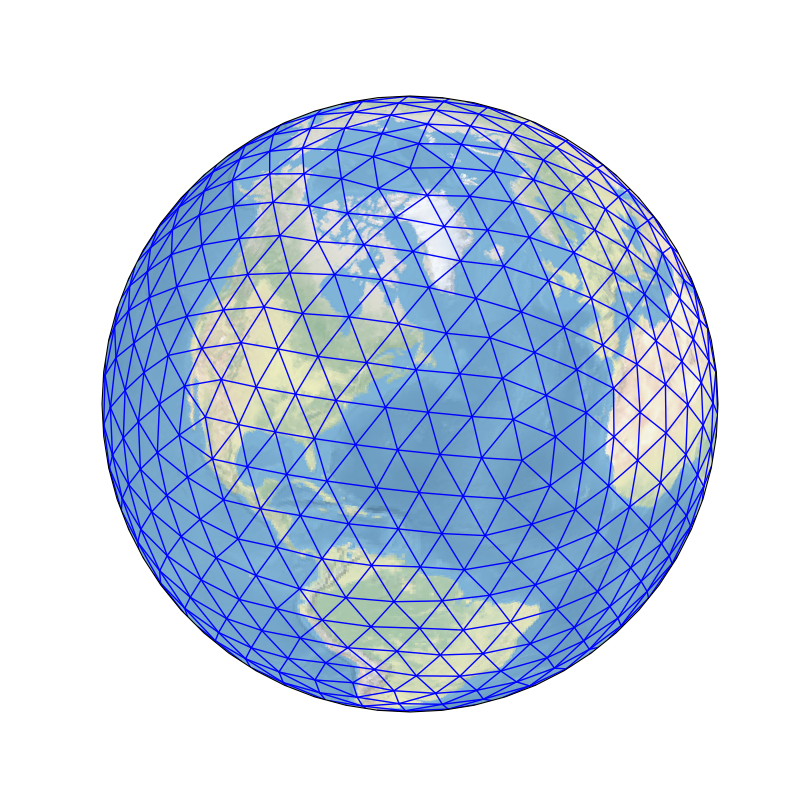
\includegraphics[width = \linewidth]{icos_pol_nopt_3_edsphere}
    \caption{Icosahedral grid}
  \end{subfigure}
  \begin{subfigure}{.3\linewidth}
    \centering
    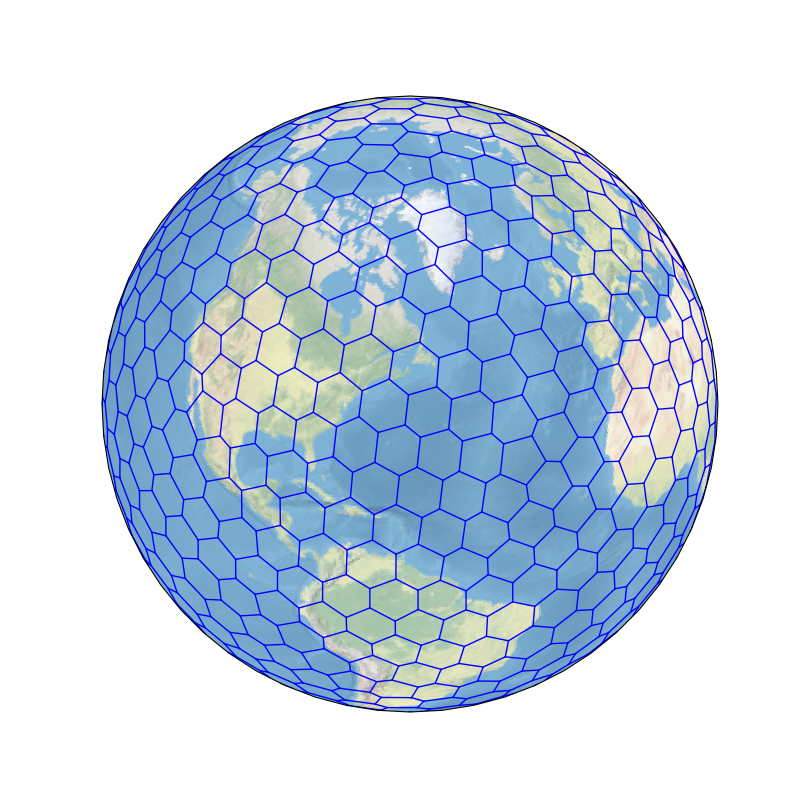
\includegraphics[width = \linewidth]{icos_pol_nopt_3_edhxsphere}
    \caption{Pentagonal/Hexagonal grid}
  \end{subfigure}
  \begin{subfigure}{.3\linewidth}
    \centering
    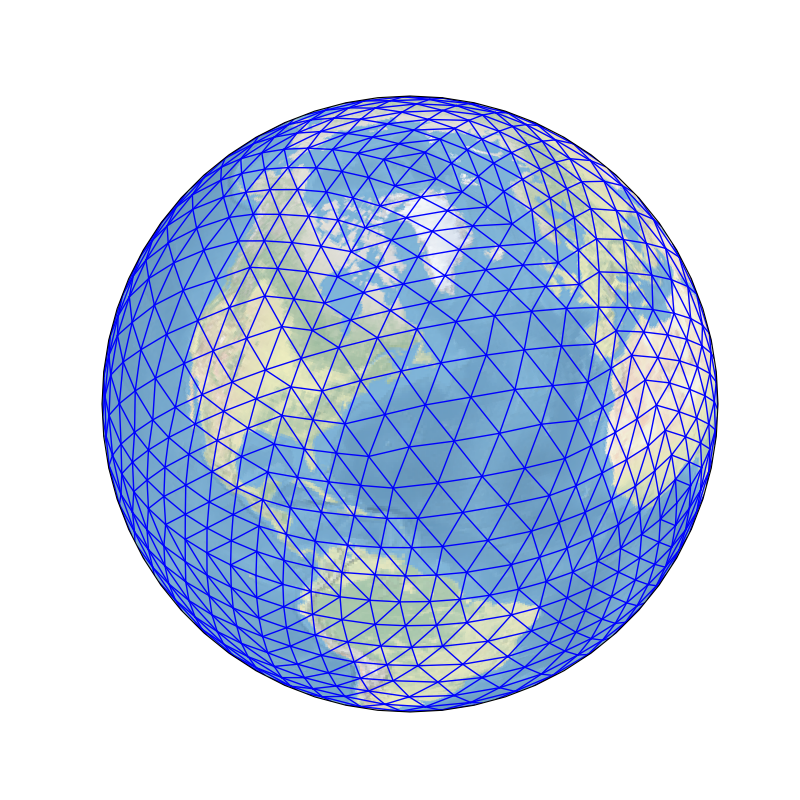
\includegraphics[width = \linewidth]{octg_pol_nopt_4_edsphere}
      \caption{Octahedral grid}
  \end{subfigure}
  \caption{Examples of spherical grids: }
\end{figure}
\citep{stan:2012} \citep{ullrich:2017}

